\documentclass[10pt,twocolumn,letterpaper]{article}

\usepackage{cvpr}
\usepackage{times}
\usepackage{epsfig}
\usepackage{graphicx}
\usepackage{amsmath}
\usepackage{amssymb}
\usepackage[breaklinks=true,bookmarks=false]{hyperref}
\usepackage[caption=false, font=footnotesize]{subfig}
\cvprfinalcopy % *** Uncomment this line for the final submission

\def\cvprPaperID{****} % *** Enter the CVPR Paper ID here
\def\httilde{\mbox{\tt\raisebox{-.5ex}{\symbol{126}}}}

\begin{document}

\title{CS280.01: Machine Learning\\ Project 1}

\author{Zhixin Piao, Yongfei Liu, Kang Zhou\\
ShanghaiTech University\\
{\tt\small { \{piaozhx, liuyf3, zhouk\}@shanghaitech.edu.cn}
}}

\maketitle

\begin{abstract}
   Marketing classification is the most common task in machine learning. In this report, we will present the whole pipeline to deal with real marketing case. Our methods can seperate into three main parts, which are data processing, modeling, and explanation respectively. In data processing, we will present some common tricks in machine learning to solve imbalance data, missing value and feautre selection problems. In modeling stage, we use some basic models to do the classification and finally ensemble all the models together to get higher perfermance. We will present some methods to select hyperparameters. At last, we want to give some explanation for our final deicison by diagnosing the weights and anasylis some common features appearing in positive coustomers. Our conclusion can give more hints to our final marketing strategies.
\end{abstract}

\section{Introduction}

\section{Data Preprocessing}

\begin{figure}[ht]
    \centering
    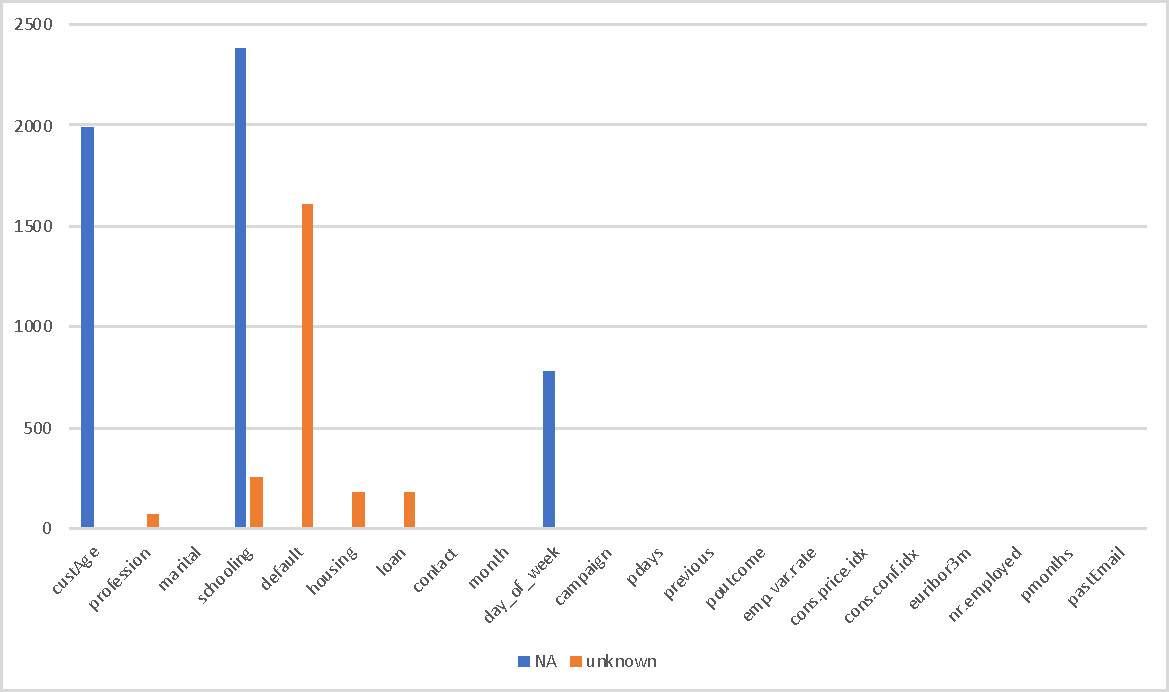
\includegraphics[width=0.5\textwidth]{img/missing.pdf}
    \caption{missing dat distirbution}
    \label{missing}
\end{figure}

\subsection{Fill missing values}
We find there are many missing values in training set, like `NA', `unknown'. we think that just remove these samples whose feature includes missing value is not a good idea because there are almost 30\% data include missing value.

Actually, most of the missing values are in `custAge', `schooling', `default' and `day\_of\_week' (details have been shown in Fig.\ref{missing}), a basic idea is fill these values with 0 or random sample some value from this attribute, but it will bring many noise data, so we deicde to select nearest sample which has real value to fill in.

\subsection{Normalization}
There are 4 type of feature: \textbf{bool}, \textbf{int}, \textbf{float} and \textbf{enum}. For int and float type, different feature has big difference of scale and region, so we should do normalization. a common normalization algorithm is \textbf{z-score}:
\begin{align*}
    z = \frac{z - \mu}{\sigma}
\end{align*}
where $\mu$ is the mean of population, $\sigma$ is the standard deviation of the population.



On the other hand, we use \textbf{one-hot code} to handle bool and enum type: if an enum feature has 4 different attribute, we will encode it into a 4 dimension vector, and each dimension correspond to an attribute.


\subsection{Feature Selection}
There are many attributes in oen sample feature, which will cause the curse of dimensionality, which means that will let model complex and hard to train, so feature selection is important.



In Fig.\ref{cor}, obviously there are some features are linearly dependent, which isn't important and should be removed. 

\subsection{Handling unbalanced data}
The final target of us is train a model to predict customer who brings profits(larger than 30). but these people are only 10\% of total train set, i.e. wanted people is too little to train a robust model, so we should create some new data to balance.

\begin{figure}[ht]
    \centering
    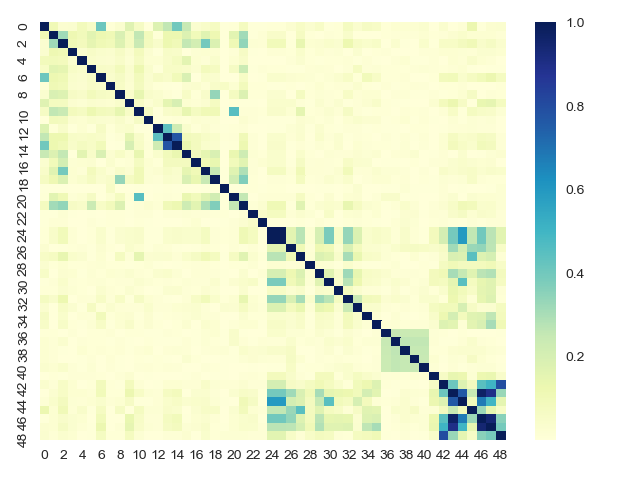
\includegraphics[width=0.5\textwidth]{img/Cor.png}
    \caption{Corelation Matirx}
    \label{cor}
\end{figure}

\begin{figure}[ht]
    \centering
  \subfloat[origin]{%
       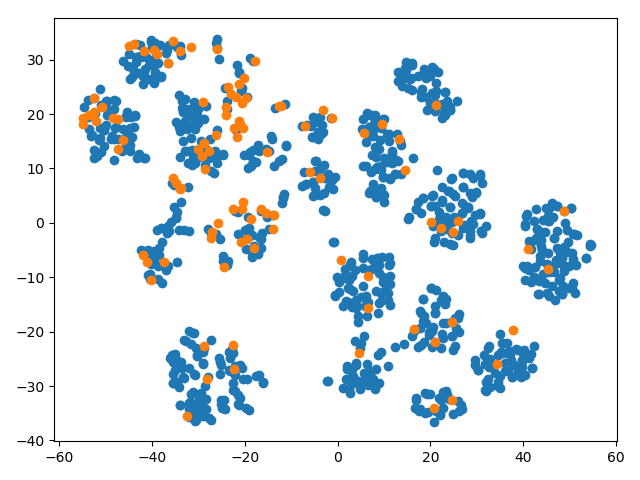
\includegraphics[width=0.45\textwidth]{img/unbalanced.png}}
    \label{1a}
  \subfloat[oversampling]{%
        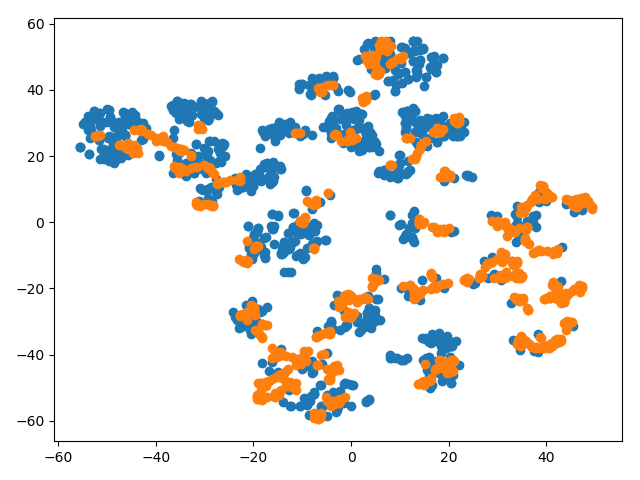
\includegraphics[width=0.45\textwidth]{img/balanced.png}}
    \label{1b}
  \caption{oversampling}
  \label{oversampling} 
  \end{figure}


\textbf{SMOTE}(Synthetic Minority Oversampling Technique) is a well known oversampling method to handle unbalanced data.

\section{Method}
Here we will presnet some basic models to solve this question independently, which includes logistic regression, svm, decision tree and random forest. At last we will introduce how to ensemble all the model together to boost our perfermances.
\subsection{Logistic Regression}
In this task, the logistic regression can solve the binary classification problems. The specific model is as following:
\begin{equation}
    P(y|x) = \sigma(y\cdot W^Tx)
\end{equation}
Once we confirm the model, we can construct some loss function to learn the parameters by stochasitc gradient descent.
\begin{equation}
    loss(y, x) = -\sum_{i=1}^{m} [y_i ln\sigma(W^Tx_i)+(1-y_i)ln(1-\sigma(W^Tx_i))]
\end{equation}
In genearlly, we can overfit the validation data because of lots of features. So we need to add some regularization term to reduce the model complexity.
So we can rewrite the loss function as:
\begin{equation}
    loss_{reg}(y,x) = loss(y, x) + \lambda W^TW
\end{equation}
Here we will explore the influence of regularization strength terms. 
\begin{figure}
    \centering
    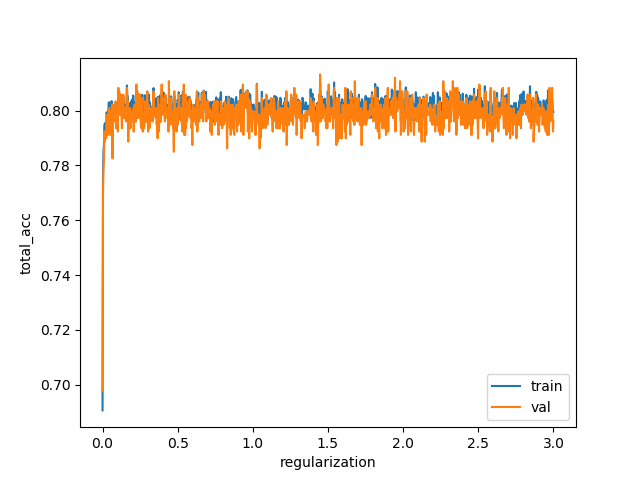
\includegraphics[width=0.5\linewidth]{img/acc_bs1_total_smote.png}
    
\end{figure}
We can see that when we set $\lambda=0.189$ to get the best perfermances.

\subsection{SVM}
The intuition of SVM\cite{SVM} is to manimize the margin, which can get more better generalization powers. Let's see mathematical equations in SVM.
\begin{align}
    min_w & \quad \frac{1}{2} W^TW \\
    s.t. &\quad y_i(W^T x_i+b) \geq 1  \quad i = 1\dots m
\end{align}

In genearlly, the data cannot be seperated in limited dimension. So we can map the data to high dimension to let it be sepearted. So we can use some kernel tricks to get better perfermances. There are several kernel function,so we will give some comparision for different kernel function.
\textbf{to post some figure in kernel function}

\subsection{Decision Tree}
The decision tree can provide a explainable model to solve problems. In this taks we have different attributes in total. We can compute the information gain to get the split results.
\begin{equation}
    Gain(D, a) = Ent(D) - \sum_{v=1}^{V} \frac{|D^v|}{|D|} Ent(D^v)
\end{equation}
In some degree, information gain can solve most of problems.But when we have lots of categories, information gain will fail. So we can use gain ratio to get more better perfermances.
\begin{align}
    &Gain\_ratio(D, a) = \frac{Gain(D,a)}{IV(a)}\\
    &IV(a) = -\sum_{v=1}^{V} \frac{|D^v|}{|D|} \log\frac{|D^v|}{|D|}
\end{align}
we always choose the most gain ratio to be our nodes. There are lost of parameters in decision tree, we will give the influence of tree depth.

% pic
\section{Explanation}


{\small
\bibliographystyle{ieee}
\bibliography{egbib}
}

\end{document}
